% === TP01 - Trabajo Practico - Diseño de procesadores ===
% David Alejandro Gonzalez Marquez
% fokerman@gmail.com
% https://github.com/fokerman/fpgaSoftcoreProgrammingCourse

\documentclass[a4paper,11pt]{article}

% Tamaño
\usepackage[a4paper]{geometry}
\geometry{top=1.5cm, bottom=1.5cm, left=2.0cm, right=2.0cm}

% Idioma y encoding
\usepackage[utf8]{inputenc}
\usepackage[spanish,activeacute]{babel}

% Fuentes
\usepackage{amsfonts}
\usepackage{amsmath}
\usepackage{amssymb} % Para tener bigstar
\usepackage{latexsym}

% Otros
\usepackage[dvips]{graphicx}
\usepackage{enumerate}
\usepackage{multirow}
\usepackage{moreverb}
\usepackage{multicol}
\usepackage{framed}
\usepackage{xspace}  % Para tener espacios luego de nuevos comandos si es necesario
\usepackage[colorlinks=false, linkcolor=black, bookmarks=false, bookmarksopen=false]{hyperref}
\usepackage{xcolor}
\usepackage{colortbl}

% Colores
\definecolor{verdeuca}{rgb}{0.0,0.48,0.54}
\definecolor{naranjauca}{rgb}{1,0.48,0.0}
\definecolor{AzulClaro}{rgb}{.31,.506,.741}
\definecolor{Gris}{gray}{0.8}
\definecolor{Celeste}{rgb}{.255,.41,.884}
\definecolor{Rojo}{rgb}{1, 0, 0}
\definecolor{a}{rgb}{0.0, 0.53, 0.74}
\definecolor{r}{rgb}{0.89, 0.0, 0.13}
\definecolor{v}{rgb}{0.0, 0.5, 0.0}
\definecolor{y}{rgb}{0.0, 0.5, 0.5}
\definecolor{rojo}{HTML}{F1521B}
\definecolor{verde}{HTML}{80CD29}
\definecolor{amarillo}{HTML}{FABC09}
\definecolor{azul}{HTML}{00ADF1}

\title{Trabajo Práctico\\ 
\large{Diseño de procesadores}}
\author{Materia: Programación de softcores en FPGAs\\
Programa de Profesoras/es Visitantes}
\date{}

\usepackage{todonotes}

\begin{document}

\maketitle

\begin{center}
    \scriptsize Material disponible en: \url{https://github.com/fokerman/fpgaSoftcoreProgrammingCourse}
\end{center}

\section{Introducción}

El objetivo de este trabajo práctico es diseñar la arquitectura de un procesador, con sus instrucciones, lenguaje ensamblador, codificaciones y características propias.
Para luego implementar dos posibles organizaciones que respeten la arquitectura diseñada.
El procesador en cualquiera de sus dos organizaciones, deben ser capaz de ejecutar programas en lenguaje ensamblador.
En este trabajo se pedirá implementar un juego tipo Simon.

\section{Enunciado}

El enunciado consta de cinco partes, la primera invita a diseñar la arquitectura de un procesador simple, similar a un modelo Von Neumann clásico.
La segunda y tercera parte desarrollan este procesador implementadolo con dos \emph{datapaths} diferentes, uno de un solo bus y una organización microprogramada,
mientras que el segundo construye un modelo donde cada instrucción se ejecuta en un ciclo de reloj.
La cuarta parte consiste en implementar el código de un juego para los dos procesadores desarrollados.
La última parte consiste en extender el soporte de la arquitectura para alguna característica particular.

En este enunciado no hay necesariamente pasos a seguir, sino referencias de todo lo que debe soportar y poder realizar el procesador que se desarrolle.
Esto implica que puede ser necesario revisitar la definición de la arquitectura en base a una alteración de la organización.
Sobre todo para hacer más simple la organización del procesador, en especial para el \emph{datapath} de un solo ciclo y el último ejercicio.

El procesador que se espera que diseñen en este trabajo debe respetar las siguientes características:

\subsection{Características mínimas}

A continuación se lista un conjunto de características que debe respetar su diseño.
En caso que lo consideren necesario puede alterar alguna de estas características, siempre que su alteración tenga mejor o mayor soporte que el original.

\begin{itemize}

\item Tamaño de palabra, operaciones y datos de 8 bits. Instrucciones de tamaño fijo de 16 bits.
\item Registros expuestos al programador, al menos 6 registros de propósito general, un registro para el PC y un registro de Flags, Carry, Negative, Overflow, Zero.

\item Modos de direccionamiento. Se debe poder soportar, dependiendo de cada instrucción, los modos de direccionamiento: inmediato, directo a registro, directo a memoria, indirecto a registro.

\item Instrucciones. Mínimamente se deben soportar las siguientes instrucciones:
\begin{itemize}
    \item Aritméticas y lógicas: Addition, Subtraction, Logic Or, Logic And, Logic Not, Compare, Logical Shift Right, Logical Shift Left. Estas deben operar mínimamente con cualquier registro de propósito general.
    \item CopyRegister: Instrucción para copiar el contenido de un registro en otro.
    \item Saltos: Jump, Jump Equal, Jump Not Equal
    \item Subrutinas: callSubrutine, ReturnSubrutine. Instrucciones para llamar a subrutinas, estas instrucciones se pueden implementar utilizando la pila o utilizando registros específicos donde almacenar la dirección de retorno.
    \item GetFlags: Instrucción que permita leer los Flags, ya sea escribiéndolos en un registro o en memoria.
    \item Memoria: writeToMem, readFormMem. Instrucciones para leer y escribir en memoria.
    \item SetRegister: Instrucción para asignar un valor inmediato a un registro.
\end{itemize}

\item Memoria de datos: 1kB, direcciones de 10 bits con direccionamiento a 8 bits.

\item Memoria de código: 1kB, direcciones de 9 bits con direccionamiento a 16bits.

\item Pila: Puede ser implementada de forma estática en una estructura no acessible por el programador o dinámica en memoria.
En cualquier caso debe soportar al menos 5 llamados a funciones anidadas.

\item Entrada/salida: El procesador dispondrá de un puerto de 4 bits de entrada y un puerto de 4 bits de salida.
Ambos puertos deben estar mapeados a memoria en alguna dirección fija designada.

\end{itemize}

\noindent \textbf{Observaciones}\\

\indent La memoria de código y de datos tienen diferentes unidades direccionables, dos unidades direccionables de datos se requieren para tener una unidad direccionable de la memoria de código.
Si bien son del mismo tamaño, una debe tener el doble de direcciones que la otra.
Esto implica que se debe tener especial cuidado cuando se considera una dirección en la memoria de datos y en la memoria de instrucciones.\\
\indent Notar que en ningún lugar se indica si la memoria de datos y código debe ser compartida. Se recomienda diseñar la arquitectura considerando que las memorias son independientes, sin embargo tienen esta libertad.\\

Las características mencionadas son las mínimas que debe cumplir la arquitectura.
Es posible agregar más instrucciones, o más registros o más puertos de entrada salida o incluso soporte para interrupciones.

\subsection{Ejercicio 1: Diseño de arquitectura}

Utilizando como base las características enunciadas en el punto anterior, se pide diseñar una arquitectura de un procesador que las respete.

\begin{itemize}
\item Proponer un nombre a su arquitectura.

\item Definir la arquitectura del procesador, documentar y describir cada una de sus características principales.

\item Definir el conjunto de instrucciones soportadas por el procesador, indicando el comportamiento de cada una.

\item Definir una codificación para cada una de las instrucciones, indicar los campos y el comportamiento que debe realizar el decodificador de instrucciones para tomar cada uno de los campos.

\item Definir un lenguaje ensamblador, indicar lo nemónicos de cada instrucción y como se indican los parámetros. El lenguaje debe incluir palabras reservas para definir constantes en memoria y resolver etiquetas.

\item Desarrollar un programa que tome un archivo de texto y construya un archivo ensamblado. El programa debe retornar otro archivo de texto codificando los bytes en caracteres hexadecimales. Este archivo se utilizará luego como entrada de la memoria de código. Se recomienda realizar el desarrollo en \texttt{Python}.

\item Implementar tres programas de ejemplo:
\begin{itemize}
 \item Un programa que realice un ciclo escribiendo los números del 1 al 10 en la memoria de datos.
 \item Un programa que lea datos de memoria previamente escritos y cuente todas las apariciones de un determinado valor \texttt{target} en un rango de memoria dado.
 \item Un programa que lea los 4 bits del puerto de entrada, interprete el valor como un numero entero, calcule el inverso aditivo y escriba el resultado en el puerto de salida.
\end{itemize}
\end{itemize}

El resultado de este ejercicio debe ser una documentación detallada del diseño de la arquitectura. Equivalente a una hoja de especificaciones o manual.

\subsection{Ejercicio 2: Organización microprogramada}

Llamaremos una organización microprogramada a una implementación clásica de un modelo de computadora con un solo bus compartido, con memorias independientes para código y datos.
La unidad de control se ocupará de activar secuencialmente las señales para realizar el ciclo de instrucción y resolver cada una de las instrucciones.

\begin{center}
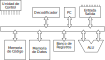
\includegraphics[scale=1]{img/orga_microprogramada.pdf}
\end{center}

\begin{itemize}
 \item Diseño del \emph{datapath}, identificar todos los registros temporales que se utilizarán y que información se almacenará en cada registro.
 
 \item Definir el ciclo de instrucciones, como se leerá una instrucción y los pasos para que sea decodificada para luego ser ejecutada.
 
 \item Definir las señales de control del \emph{datapath}, para esto recorrer instrucción por instrucción caracterizando las señales que serán utilizadas en cada flujo de control.
 
 \item Diseñar la secuencia de activación de señales para resolver cada instrucción. Se recomienda utilizar una memoria dentro de la unidad de control para almacenar las codificaciones.
 Si son muchas señales es recomendable implementar un programa ayude a construir la entrada para la memoria.
 
 \item Implementar en \texttt{Verilog} el componente ALU, realizar un \emph{testbech} de todas las operaciones que debe soportar.
 
 \item Implementar en \texttt{Verilog} el componente PC, realizar un \emph{testbech} que pruebe como es incrementado y los valores que toma.
 
 \item Implementar en \texttt{Verilog} el banco de registros, realizar un \emph{testbech} de la escritura y lectura de registros.
 
 \item Implementar en \texttt{Verilog} los módulos de memoria, tanto de código como de datos o los dos simultáneamente. Considerar que la memoria debe tener en cuenta las señales para controlar los puertos de entrada/salida mapeados a memoria. Realizar un \emph{testbech} que pruebe escrituras y lecturas en memoria, teniendo en cuenta los puertos mapeados.
 
 \item Implementar en \texttt{Verilog} el módulo que permite exponer o recibir datos de entrada/salida. Debe responder a las mismas señales que la memoria, ya que está mapeado a memoria. Realizar un \emph{testbech} que pruebe leer y escribir en un puerto de entrada/salida, se debe poder soportar tanto escribir en el puerto de lectura, como leer del puerto de escritura.
 
 \item Implementar en \texttt{Verilog} el \emph{datapath} y la unidad de control del sistema. Identificar todas las conexiones entre los módulos. Tener en cuenta el criterio de nombres utilizado, tanto para las señales internas como externas de cada módulo. Además ordenar las señales de forma que sea simple identificar un error en el funcionamiento.
 
 \item Ejecutar los programas realizados en el ejercicio anterior y probar su correcto funcionamiento.  
\end{itemize}

El resultado de este ejercicio debe ser un conjunto de archivos \texttt{Verilog} con el código implementado, archivos con los programas \texttt{asm} desarrollados y ejecutados, y un informe explicando toda la implementación del procesador.

\subsection{Ejercicio 3: Organización en un solo ciclo}

\begin{center}
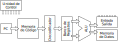
\includegraphics[scale=1]{img/orga_oneclock.pdf}
\end{center}

\begin{itemize}
 \item Diseño del \emph{datapath}, identificar todos los flujos de instrucciones y las dependencias entre cada uno de los componentes. Identificar que elementos del circuito cambian en el ciclo de reloj.
 
 \item Diseñar el flujo para incrementar y modificar el PC.
 
 \item Diseñar el flujo de decodificación de instrucciones, identificando que señales deben ir a la unidad de control y cuales deben ir al banco de registros.
 
 \item Diseñar el banco de registros de forma de soportar la cantidad de lecturas y escrituras simultaneas que hagan falta.
 
 \item Diseñar el flujo de datos desde la ALU u otras partes del \emph{datapath} a el lugar donde se escriba el resultado de una operación, ya sea memoria, entrada salida o el mismo banco de registros.
 
 \item Diseñar el flujo de datos de la unidad de control y como las diferentes señales deben llegar a cada uno de los módulos del \emph{datapath}. Agregar los multiplexores y decodificadores necesarios para resolver los flujos de datos y control.
 
\item Implementar en \texttt{Verilog} cada uno de los componentes diseñados y su \emph{datapath}. En todos los casos realizar \emph{testbech} de las diferentes partes.
 
 \item Ejecutar los programas realizados en el ejercicio anterior y probar su correcto funcionamiento.
\end{itemize}

El resultado de este ejercicio debe ser un conjunto de archivos \texttt{Verilog} con el código implementado, archivos con los programas \texttt{asm} desarrollados y ejecutados, y un informe explicando toda la implementación del procesador.

\subsection{Ejercicio 4: El juego}

Desarrollar el código ensamblador del juego electrónico \textbf{Simon}. Las 4 salidas del puerto de salida serán conectadas a leds, mientras que las 4 entradas del puerto de entrada serán conectadas a pulsadores. Un pulsador y un led será utilizado para cada color del juego. Para reiniciar el juego se deberá presionar al menos dos pulsadores simultáneamente.

\begin{center}
 
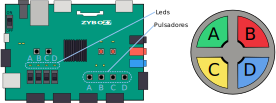
\includegraphics[scale=0.5]{img/zyboZ7_simon.pdf}
\end{center}

\begin{itemize}
 \item Desarrollar el código ensamblador para la arquitectura implementada. Este código debe funcionar de forma equivalente en las dos organizaciones de procesador implementadas.

 \item Desarrollar el código \texttt{Verilog} para conectar los puertos de entrada/salida del procesador a los leds y pulsadores.
 
 \item Desarrollar el código de configuración de \emph{constrains} para conectar el circuito a los puertos correspondientes de la placa de pruebas.
 
 \item Probar experimentalmente el código desarrollado en las dos organizaciones de procesador implementadas. Tener en cuenta que la temporización de los eventos en ambas organizaciones será diferente, por lo que es fundamental dejar el código ensamblador preparado para alterar las constantes de temporización en el caso de ser necesario.
\end{itemize}

El resultado de este ejercicio consistirá en probar su implementación en la placa FPGA. Se espera que puedan jugar al juego y recordar al menos 5 colores.

\subsection{Ejercicio 5: Extensión de la Arquitectura}

En este ejercicio se propone extender la arquitectura con al menos una de las siguientes características:

\begin{enumerate}[A.]
 \item \textbf{Soporte para interrupciones}\\
 Al menos se debe poder soportar una señal de interrupción que ejecute una sola rutina de código en una posición fija de memoria.
 La interrupción se debe generar ante el cambio de algún bit en un registro específico de entrada/salida.
 \item \textbf{Soporte para protección de memoria}\\
 Al menos el procesador debe soportar dos áreas de memoria distinguidas entre supervisor y usuario. El acceso a el área del supervisor estará limitado a código que ejecute con modo supervisor.
 Salir y entrar en modo supervisor solo se podrá hacer mediante un llamado específico a una rutina del sistema. La protección será válida tanto para lecturas y escrituras de datos como para ejecución de código.
 \item \textbf{Soporte para pila}\\
 Se debe dar soporte para las instrucciones de \texttt{push} y \texttt{pop} usando una pila implementada en memoria. Además estas instrucciones debe soportar tres modos de direccionamiento: inmediato, directo a registro y directo a memoria.
\end{enumerate}

El resultado de este ejercicio consistirá en la documentación de la especificación del soporte propuesto. Se debe adjuntar en la documentación detalles de como se implementaría en las dos organizaciones presentadas en este trabajo práctico.

\section{Entrega}

Este trabajo práctico tendrá cuatro entregas o presentaciones. Las fechas de las entregas serán fijadas en el transcurso de la materia.
En todos los casos se solicitará entregar un archivo pdf con el informe de la entrega correspondiente, con toda la información y código incluido.
Adicionalmente los archivos de código deben ser adjuntados en otro archivo comprimido, junto con toda la información o documentación que se requiera para entender su solución particular.

\begin{itemize}
\item Entrega 1: Diseño de arquitectura\\
Documentación de la arquitectura, definiciones de tamaños, parámetros. Descripción completa del conjunto de instrucciones con sus respectivos modos de direccionamiento. Detalle de la codificación de todas las instrucciones. Programa ensamblador y ejemplos de su funcionamiento.
\item Entrega 2: Organización microprogramada\\
Documentación del \emph{datapath} completo. Descripción de su funcionamiento, ciclo de instrucción y flujo de ejecución de instrucciones. Código \emph{Verilog} completo con su \emph{testbech}.
\item Entrega 3: Implementación en un solo ciclo\\
Documentación del \emph{datapath} completo. Descripción de su funcionamiento, ciclo de instrucción y flujo de ejecución de instrucciones. Código \emph{Verilog} completo con su \emph{testbech}.
\item Entrega 4: El juego\\
Implementación del juego en ensamblador. Pruebas de su funcionamiento en las dos organizaciones. Código \texttt{Verilog} para probarlo.
\item Entrega 5: Extensión de la Arquitectura\\
Esta entrega se presentará el último día de clases como parte de la evaluación final de la materia.
\end{itemize}

\end{document}
